\section{Measured matrices and coherent choices on Maharam slabs}
\label{sec:slabs}

Let $\mathcal R$ be a countable nonsingular Borel equivalence relation
on a standard probability space $(V,\mu)$. All measurable objects are
understood modulo null sets, with Borel representatives. Our convention
for the multiplicative Radon--Nikodym cocycle is
\begin{equation}
 d\mu(w)=\omega(v,w)\,d\mu(v)
 \label{slab:cocycle}
\end{equation}
along partial isomorphisms $v\mapsto w$ with graph in $\mathcal R$.
An invariant null set can be removed so that the cocycle identities hold
on the resulting relation.

Consider a measurable system $T$ of Hermitian contractions with zero
diagonal on the spaces $\ell^2([v]_{\mathcal R})$. The system is
\emph{principal}: the indices are the points of an equivalence class,
with one index for each point. On changing the root within a class, the
matrices agree up to conjugation by diagonal unitaries. Suppose their
entries are supported on an undirected Borel graph $\mathcal G$ in
$\mathcal R$, of degree at most a fixed finite number $D$, and suppose
that for a fixed $J\geq1$,
\begin{equation}
 J^{-1}\leq\omega(v,w)\leq J
 \quad\text{on every edge of }\mathcal G.
 \label{slab:edge-cocycle}
\end{equation}
A measurable coloring of $V$ defines $T_{\mathrm{pav}}$ by retaining
entries whose two indices have the same color and setting the other
entries to zero. For a function of an orbit matrix, its diagonal entry
at the root $v$ is denoted by a subscript $vv$.

\begin{theorem}[One-sided measured paving]
\label{thm:measured-paving}
There is a universal constant $K\geq1$ with the following property.
Suppose $T$, $\mathcal R$, $\mathcal G$, and $\omega$ satisfy the preceding
assumptions. Let $b>0$, and choose a positive integer $r$ such that
\begin{equation}
 2\sqrt{2/r}+2/r<b.
 \label{slab:r-choice}
\end{equation}
For every $\sigma>0$ and $\rho>0$, there is a measurable coloring of $V$
with $r+1$ colors for which
\begin{equation}
 \int_V \bigl((T_{\mathrm{pav}}-(Kb+\sigma)\one)_+^2\bigr)_{vv}
 \,d\mu(v)<\rho.
 \label{slab:measured-conclusion}
\end{equation}
\end{theorem}

We use the constants $K$ and $C$ of Lemma~\ref{lem:buffered-pin}.
This section constructs choices that are coherent along the height
coordinate of the Maharam extension: the finite buffered inequality
selects a color at a lifted vertex, but a paving of the base requires
the same choice at every height above that vertex. The proof of
Theorem~\ref{thm:measured-paving} is completed by the sparse pinning and
descent argument in the next section. All constants called uniform in
this section may depend on $D,J,r,b$ and the fixed matrix system, but
not on a partial assignment or on the endpoints of a slab. Constants
for a single fixed slab will be identified separately.

\subsection{Invariant measure and weighted polynomial systems}

For the Maharam extension, see \cite{Maharam64} and the formula in
\cite[Section~2, before Theorem~2.1]{RoySamorodnitsky06}; the multiplicative
coordinate there is $y=e^{-s}$ in our convention. We verify invariance
in the present cocycle notation before developing the slab construction.
The Maharam extension has vertices
$u=(v,s)\in V\times\R$ and relates
$(v,s)$ to
\[
 (w,s+\log\omega(v,w)),\qquad (v,w)\in\mathcal R.
\]
Projection to $V$ is injective on each lifted orbit: the cocycle
identities fix the height over $w$ uniquely. The measure
\[
 d\widetilde\mu(v,s)=d\mu(v)e^{-s}\,ds
\]
is invariant along this relation. Indeed, writing
$s'=s+\log\omega(v,w)$, Equation~\eqref{slab:cocycle} gives
\[
 d\mu(w)e^{-s'}ds'=\omega(v,w)d\mu(v)
       \frac{e^{-s}}{\omega(v,w)}\,ds=d\mu(v)e^{-s}ds.
\]
Consequently the mass-transport identity is
\begin{equation}
 \int \sum_y F(u,y)\,d\widetilde\mu(u)
 =\int \sum_u F(u,y)\,d\widetilde\mu(y)
 \label{slab:mass-transport}
\end{equation}
for nonnegative measurable transports along the lifted relation, and
for integrable complex transports. The identity remains true after
restricting both endpoints to a slab or to any further measurable
subset. To justify it, decompose the countable Borel relation into
countably many graphs of partial Borel isomorphisms, using the
countable-section decomposition theorem and its application to the
inverse relation. On each lifted graph it is precisely the preceding
change of variables; summing the graphwise identities proves the
claim. The scalar polynomial data used below are invariant under the
allowed diagonal-unitary gauges, so they define transports without any
choice of gauge.

Fix a bounded interval $I$ and restrict the lifted graph and matrices
to $V\times I$. A partial assignment on the base $V$ specifies a color
at some vertices. At unassigned vertices let $t_{vi}=1/r$ for every
$i$ and let $c_v=b$; at assigned vertices let $(t_{vi})_i$ be the
corresponding point mass and let $c_v=Kb$. Lift these data unchanged in
$s$, and set
\begin{equation}
 d_u=e^s\quad(u=(v,s)),\qquad
 W=d^{1/2}Td^{1/2},\qquad a_u=d_uc_v.
 \label{slab:weighted-system}
\end{equation}
The weight $d_u=e^s$ cancels the density $e^{-s}$ of the invariant
measure: an absolute spectral cost integrated against
$d\widetilde\mu$ is its normalized cost, divided by $d_u$,
integrated against $d\mu\,ds$. This will make long slabs comparable
by ordinary averages over height.
We use the finite mixed polynomials and local data of
Lemma~\ref{lem:local-data} with these matrices and penalties.
A prospective buffered pin at an unassigned lifted vertex fixes its
color and replaces its penalty $bd_u$ by $Kbd_u$. During comparisons
we also allow arbitrary vertex deletions and single lifted-vertex
changes; these intermediate configurations need not arise from a base
assignment. Distances are always taken in the original restricted
lift of $\mathcal G$, including edges whose entries have subsequently
been set to zero.

All finite principal systems in a fixed slab, and all their prospective
pins, have their roots and poles in a common interval $[-B,B]$.
For example, an enlarged value of
$\sup_u a_u+r\norm{W}$ is sufficient: apply
Lemma~\ref{lem:stability} to the two half-planes beyond the numerical
ranges of the determinant matrices. The same conclusion holds if
some cross edges are cut or interpolated as below, with an enlarged
fixed-slab bound.

There are also estimates which do not depend on the slab.
The residue formula in Lemma~\ref{lem:local-data}, together with
$d_y/d_u\leq J$ on edges, gives
\[
 a_u\leq Kbd_u,\qquad
 \sum_j\nu_{u,j}
 \leq \sum_y\abs{W_{uy}}^2
 \leq Jd_u^2\sum_y\abs{T_{uy}}^2
 \leq Jd_u^2.
\]
They hold for each pin alternative as well. They continue to hold
under the cuts and real edge interpolations used later, since these
only decrease the absolute values of the entries. The second-moment
formula for $\gamma_u$ and the arrow representation therefore give a
constant $C_{\mathrm{loc}}$ such that
\begin{equation}
 m_u\leq C_{\mathrm{loc}}d_u,\qquad
 0\leq\ell_u\leq C_{\mathrm{loc}}d_u,\qquad
 0\leq\ell_{u,i}'\leq C_{\mathrm{loc}}d_u.
 \label{slab:local-bounds}
\end{equation}
For the last two estimates, adding the off-diagonal arrow to
$(-a_u)\oplus S$ changes the trace of the positive part by at most the
trace norm of that arrow, namely $2(\sum_j\nu_{u,j})^{1/2}$.
The positive-part trace variational formula proves this estimate;
interlacing gives its nonnegative sign. Here and below $h_i'$ denotes
the buffered pin, rather than a derivative.

\subsection{Locality and infinite bounded slabs}

\begin{lemma}[Local limits on a bounded slab]
\label{lem:slab-limits}
On each bounded slab, the finite local functions
$h_u,G_u,h_{u,i},h_{u,i}',R_{u,i}$, the probability and residue
measures, and the data $m_u,\ell_u,\ell_{u,i}'$ have unique limits as
finite graph balls increase to a component. They are measurable and
independent of the exhaustion, and the local Cauchy-transform and
Poisson-transform identities pass to the limits.
Their supports have a common fixed-slab bound, and
Equation~\eqref{slab:local-bounds} continues to hold.

The Laurent coefficients through order $k$ of $h_u/z$, $zG_u$,
$h_{u,i}/z$, $h_{u,i}'/z$, and $R_{u,i}$, and the moments of
$\gamma_u$ through order $k$, depend only on the data within graph
distance $k$ of $u$. The same assertion holds for coefficients of
logarithmic derivatives under data perturbations, with the local
perturbation directions included in the data. It remains valid under
arbitrary deletion configurations.

At an unassigned vertex the buffered pin inequality
of Lemma~\ref{lem:buffered-pin} holds for these infinite local data.
If every base vertex is unassigned, then $m_u=0$ on every bounded slab.
\end{lemma}

\begin{proof}
We first establish locality directly at the level of formal Laurent
series, so that the assertion does not depend on any limiting
argument. For a finite principal set $Q$ and $v\in Q$, put
$H_{v,Q}=h_{v,Q}/z$. Expanding the determinant expectation according
to the singleton or nontrivial permutation cycle containing $v$
gives
\begin{equation}
 H_{v,Q}=1+\frac{a_v}{z}
 -\sum_{\substack{C\ni v\\ |C|\geq2}}
 w_Cz^{-|C|}
 \prod_{x\in C\setminus\{v\}}H_{x,Q(x)}^{-1}.
 \label{slab:local-expansion}
\end{equation}
Here $w_C$ is the cycle weight in Equation~\eqref{poly:cycle-weight}.
Delete $v$ first and then the other vertices of $C$ in a fixed order;
$Q(x)$ denotes the principal set remaining just before $x$ is
deleted. The inverse quotients in the product telescope to
$f_{Q\setminus C}/f_{Q\setminus\{v\}}$ after the displayed powers of
$z$ are accounted for. Each oriented permutation cycle is counted
once, with the convention of the finite expansion.

All series $H$ have constant term $1$. A coefficient of order at most
$k$ in a term coming from a cycle of length $l$ uses only coefficients
through order $k-l$ in its inverse factors. Induction on $k$ now proves
the radius-$k$ locality assertion: the cycle has length at most $k$,
and the further radii of the needed factors stay within distance $k$
of $v$. Formal inversion, multiplication, and differentiation preserve
this property. This proves locality for all the listed series and
for their perturbation derivatives, including complex perturbations;
only the algebraic finite polynomial identities were used.
The expansion of $zG_v$ is the moment expansion of $\gamma_v$, proving
the moment assertion.

For real data, the measures $\gamma_v$ are probability measures with
support in the common compact interval $[-B,B]$. The residue measures
have support there and bounded mass for each fixed vertex, uniformly
in the finite principal subset. Locality stabilizes all their moments:
for the residue measure use the Laurent expansion of
$h_v(z)=z+a_v-\int(z-x)^{-1}\,d\nu_v(x)$. Compact-support moment
determinacy proves unique weak convergence. It also gives locally
uniform convergence of $h_v,G_v$ and their pin alternatives on
$\C\setminus[-B,B]$, in particular on the upper half-plane. Their
limits satisfy $\operatorname{Im}h_v(z)\geq\operatorname{Im}z$.

For the finite spectral-shift functions $\xi_h$, we have
$0\leq\xi_h\leq1$. Every weak-* subsequential limit therefore has
these bounds. The identity
\[
 \pi^{-1}\arg h(x+i\eta)=(P_\eta*\xi_h)(x)
\]
passes to the limit, since the Poisson kernel belongs to $L^1(\R)$
and the analytic functions converge. Poisson approximation uniquely
determines the limit function from these identities. Thus the entire
sequence converges weak-*; all functions vanish above $B$, so their
integrals over the positive axis converge. The integrals defining $m$
also converge by the compact support of $\gamma$. Apply this reasoning
to every pin alternative. The inequalities in
Equation~\eqref{slab:local-bounds} and Lemma~\ref{lem:buffered-pin}
pass to the limit, the latter because there are only finitely many
choices of color.

Finite graph balls and the corresponding finite polynomial
computations are measurable in the countable Borel relation.
Their limits are therefore measurable. The same construction applies
to single-vertex response functions indexed by pairs in an orbit.
Components disconnected in the distance graph do not affect these
local functions, so they can be treated separately. Throughout this
construction the heights and weights are absolute on the lifted
orbit; they are not reset when the root changes.

Finally suppose all vertices are unassigned. On a finite set $Q$,
the weighted polynomial at common argument $z$ is $\prod_{v\in Q}d_v$
times the unweighted mixed polynomial for $T$, with zero penalties,
evaluated at the tuple $(b+z/d_v)_{v\in Q}$. Its multiaffine Taylor
coefficients at the constant tuple $b$ are the corresponding smaller
principal polynomials evaluated at $b$. All are strictly positive by
Equation~\eqref{slab:r-choice} and Lemma~\ref{lem:mss-paving},
including the empty polynomial $1$. Hence the weighted polynomial is
strictly positive for every real $z\geq0$. All its roots are real,
so its local spectral measures have no positive support. Taking the
local limits gives $m_u=0$.
\end{proof}

\subsection{Uniform comparison under far deletions}

At an unassigned vertex of a slab define the normalized tuple
\begin{equation}
 \mathcal D^I(v,s)=e^{-s}
 \bigl(m_{(v,s)},\ell_{(v,s)},
       (\ell_{(v,s),i}')_{1\leq i\leq r}\bigr).
 \label{slab:normalized-data}
\end{equation}
We use the sum of absolute values as its norm. The superscript
records the slab, and will be omitted when the ambient configuration
is clear.

\begin{lemma}[Far-deletion comparison]
\label{lem:far-deletion}
Consider any bounded slab containing $V\times[0,1]$, any base partial
assignment, and any further measurable restriction that retains the
central vertices being tested. Deleting a measurable set of vertices
at heights $s>R$, or at heights $s<-R$, changes the tuple
in Equation~\eqref{slab:normalized-data} by an amount tending to zero
in $L^1(d\mu\,ds)$ on the central unassigned band as $R\to\infty$.
The convergence is uniform in the slab, the partial assignment, and
the deletion set. The same conclusion holds for the union of a far
high set and a far low set.
\end{lemma}

\begin{proof}
We prove the analytic comparisons first and then recover the integral
data. The transform $G$ determines the local probability measure;
$h=1/G$ and $R_i=h_i/h$ then determine the parent and pinned spectral
shifts. For high deletions we test their integrated differences against
bounded complex directions and express a single deletion response as
a logarithmic derivative. Stability bounds that derivative independently
of height. We transport its local Laurent coefficients and use analytic
uniqueness to recover the whole-deletion response. Low deletions instead
cut a matrix of small norm. All pre- and post-deletion systems use the same absolute
heights, penalties, and retained probabilities.

\paragraph{High deletions and test directions.}
Write $D$ for a set above height $R$, with $R>1$. Then
$\widetilde\mu(D)\leq e^{-R}$. For upper-half-plane arguments $z$ we
claim
\begin{align}
 \int_{\mathrm{central}}
 \abs{G_v^{\mathrm{pre}}(z)-G_v^{\mathrm{post}}(z)}
 \,d\widetilde\mu(v)
 &\leq C(z)\widetilde\mu(D), \label{slab:high-G}\\
 \int_{\substack{\mathrm{central}\\\mathrm{unassigned}}}
 \abs{R_{v,i}^{\mathrm{pre}}(z)-R_{v,i}^{\mathrm{post}}(z)}
 \,d\widetilde\mu(v)
 &\leq C(z)\widetilde\mu(D). \label{slab:high-R}
\end{align}
Here $v$ denotes a lifted vertex, and $R_{v,i}=h_{v,i}/h_v$ uses the
pin with unchanged penalty. The constants are bounded uniformly for
$z$ in upper-half-plane compact sets, independently of the slab and
assignment.

It suffices to bound the integral of each complex difference against
an arbitrary measurable direction $\lambda(v)$ with
$\abs{\lambda(v)}\leq1$, supported on the tested set. For the first
comparison perturb $Y_v$ by $\zeta\lambda(v)$. For the second, fix a
color $i$ and add $\zeta\lambda(v)$ to its probability at every tested
unassigned vertex, leaving the other probabilities unchanged. For
this second perturbation, first use unnormalized weights in the
polynomial sum. Equivalently, normalize the weights at each vertex
and multiply the resulting polynomial on $Q$ by
$\prod_{v\in Q}(1+\zeta\lambda(v))$. These additional factors cancel
in the quotient deleting one high vertex $u$, since
$\lambda(u)=0$.

In a finite principal system, differentiation of the numerator and
denominator yields
\begin{equation}
 U_u(z):=\left.\partial_\zeta\log h_u(z;\zeta)\right|_{\zeta=0}
 =\sum_{v\ \mathrm{tested}}\lambda(v)
   \bigl(\mathcal B_v^{\mathrm{pre}}(z)
        -\mathcal B_v^{\mathrm{post}(u)}(z)\bigr),
 \label{slab:derivative-identity}
\end{equation}
where $\mathcal B_v=G_v$ or $R_{v,i}$, respectively, and
$\mathrm{post}(u)$ means deletion of this one vertex. For the
probability perturbation, the unnormalized derivative at $v$ is
exactly the polynomial with $v$ pinned to color $i$; its logarithmic
derivative is $R_{v,i}$. The cancellation just noted allows us to
estimate $h_u(z;\zeta)$ using the normalized determinant formula in
Lemma~\ref{lem:stability}.

\paragraph{A uniform bound for the logarithmic derivative.}
Fix $\eta>0$ and upper arguments with $\operatorname{Im}z\geq\eta$.
There is a disk $\abs{\zeta}<s_*$, independent of the slab, directions,
finite principal set, and assignment, on which
$\operatorname{Im}h_u(z;\zeta)\geq\eta/2$.
For the diagonal perturbation, the relevant determinant matrices
change by norm at most $\abs{\zeta}$.
For the probability perturbation, all tested vertices initially have
probabilities $1/r$. The normalized probabilities have analytic square
roots near these positive values on a common disk
$\abs{\zeta}<c/r$, and their changes are bounded by a constant times
$\abs{\zeta}$ on a smaller disk. Square roots at all other vertices
are unchanged, including the zero probabilities at assigned vertices.
Every changed matrix entry is incident to the central band, and its
other endpoint has height in $[-\log J,1+\log J]$ by
Equation~\eqref{slab:edge-cocycle}. Bounded row and column sums,
using the degree bound, therefore bound the entire matrix perturbation
by $C\abs{\zeta}$, uniformly in the enclosing slab.

The initial determinant matrices are Hermitian. Taking $s_*$ small
enough, their perturbed numerical ranges have imaginary parts less
than $\eta/2$ in absolute value. Lemma~\ref{lem:stability} gives
nonvanishing when all diagonal variables have imaginary part greater
than $\eta/2$, for every principal subset. In the diagonal-perturbation
case, regard the shifts as perturbations of the penalties. The final
quotient at the unperturbed vertex $u$ is monic affine in $Y_u$; its
zero therefore has imaginary part at most $\eta/2$. Evaluating at the
common argument $z$ proves the asserted lower bound on the imaginary
part of $h_u(z;\zeta)$.

A holomorphic logarithm on the $\zeta$ disk now has imaginary part
between $0$ and $\pi$. The harmonic gradient estimate and the
Cauchy--Riemann equations give
\begin{equation}
 \abs{U_u(z)}\leq C(\eta).
 \label{slab:uniform-U}
\end{equation}
The bound does not involve the size of $h_u$ or the height of $u$.
Thus high vertices with arbitrarily large real weights cause no loss
of uniformity.

For each fixed bounded enclosing slab, we also need uniform control
near infinity. On a common small $\zeta$ disk all perturbed determinant
matrices then have a uniform norm bound. Choose $B'$ larger than this
bound and larger than every real support bound, with positive slack.
For $\abs{z}>B'$, use the half-plane in the direction $z/\abs z$
strictly beyond the matrix norm bound. The affine quotient belongs
to a rotated half-plane through the origin, so the same logarithmic
argument gives a uniform bound for $U_u$ there. This bound and $B'$
may depend on the fixed slab; they are uniform in its principal
subsets, directions, and assignment states. In particular the
functions $U_u$ are analytic and locally bounded on
\begin{equation}
 \Omega=\C^+\ \cup\ \{z:\abs z>B'\},
 \label{slab:normal-domain}
\end{equation}
and are bounded near the removable point at infinity.

As finite balls around $u$ increase, normal families give
subsequential locally uniform limits on $\Omega$, also near infinity.
The locality in Lemma~\ref{lem:slab-limits}, applied to perturbation
derivatives, stabilizes every Laurent coefficient at infinity.
All subsequential limits therefore have the same Laurent series and
coincide by the identity theorem on the connected domain $\Omega$.
This defines a unique measurable function $U_u$ for infinite
components, retaining Equation~\eqref{slab:uniform-U}.

The endpoint functions $\mathcal B_v$ are also analytic on $\Omega$,
with removable values at infinity. At central vertices they are
uniformly bounded on upper-half-plane compact sets. Indeed the
residue representation gives
\[
 \abs{h_{v,i}(z)}\leq\abs z+a_v+
       \frac{\sum_j\nu_{v,i,j}}{\operatorname{Im}z},
 \qquad \operatorname{Im}h_v(z)\geq\operatorname{Im}z,
\]
and the central residue masses and penalties are uniformly bounded.
The same statements hold after deletions.

\paragraph{Recovering the whole-deletion response.}
Let $H_*(z)$ be the integral against $\lambda(v)$ of the difference
between the endpoint functions before and after deleting all of $D$.
The preceding bounds show that $H_*$ is analytic on $\Omega$, including
at infinity. We do not sum individual analytic responses over an
entire orbit. Instead we first match their local Laurent coefficients.

For each integer $k\geq1$, partition $D$ measurably into finitely many
batches such that distinct vertices of a batch have distance greater
than $2k$ in the enclosing graph, and delete the batches in order.
The required finite Borel coloring exists for every bounded-degree
Borel graph and each finite-distance graph power \cite{KST99}. For completeness,
choose a countable family of Borel binary labels separating points;
assign each vertex a finite prefix long enough to distinguish it from
its finitely many neighbors. These prefixes give a countable proper
Borel coloring. Process the countably many color classes in order,
recoloring each class with a palette of size one more than the degree
bound and avoiding the previously assigned neighbor colors. Each
class is independent, so this is a proper finite Borel coloring.

For each batch use the single-deletion logarithmic derivative in the
configuration just before that batch, and put
\[
 S_k(z)=\sum_{\mathrm{batches}}\int_{\mathrm{batch}}
 U_u^{\mathrm{pre}}(z)\,d\widetilde\mu(u).
\]
Because the batches partition $D$, Equation~\eqref{slab:uniform-U}
gives the locally uniform bound
$\abs{S_k(z)}\leq C(z)\widetilde\mu(D)$ on $\C^+$, independent of
$k$ and of the number of batches. There is a common fixed-slab bound
near infinity as well.

The Laurent coefficients of $S_k$ and $H_*$ agree through order $k$.
To see this, first apply Equation~\eqref{slab:derivative-identity} to
one deletion. At these orders only vertices within distance $k$ of
the deletion can contribute, by Lemma~\ref{lem:slab-limits}; hence
this coefficient identity on an infinite component is verified in a
sufficiently large finite neighborhood. Within one batch the
coefficient change at a tested vertex is the sum of the single
changes in the pre-batch configuration, because at most one batch
vertex belongs to its radius-$k$ neighborhood. Sum this coefficient
identity over the tested vertices and use
Equation~\eqref{slab:mass-transport} to move the sum to the deletion
vertices. The transports are integrable: for the fixed slab and fixed
order their coefficients are bounded, and their supports have a
uniform finite ball-size bound. The analytic bounds near infinity
justify interchanging coefficients and integrals. Finally sum over
the batches; the successive endpoint changes telescope to $H_*$.

Apply normal families to $S_k$ on $\Omega$ with its removable point at
infinity. Every subsequential limit has every Laurent coefficient of
$H_*$, since the first $k$ coefficients agree for each $k$. The identity
theorem shows that this limit is $H_*$ throughout $\Omega$.
It follows that $\abs{H_*(z)}\leq C(z)\widetilde\mu(D)$ on $\C^+$,
with the slab-independent constants already established there.
The fixed-slab compactness near infinity has thus transferred the
uniform upper-half-plane bound; it has not supplied a spectral-support
bound uniform over slabs.
For each fixed target $z$, choosing the measurable complex sign
$\lambda$ of the endpoint difference proves
Equations~\eqref{slab:high-G} and~\eqref{slab:high-R}.

At central vertices $h_v$ and $h_{v,i}$ are bounded uniformly on
upper-half-plane compact sets. The identity
$h^{\mathrm{pre}}-h^{\mathrm{post}}
=h^{\mathrm{pre}}h^{\mathrm{post}}(G^{\mathrm{post}}-G^{\mathrm{pre}})$
therefore gives the same $L^1$ comparison for $h$.
Then $h_i=hR_i$ gives the comparison for every $h_i$ on the central
unassigned set. Adding the unchanged shift $(K-1)a_v$ gives it for
$h_i'$ as well.

\paragraph{Low deletions.}
Suppose now that $D$ lies below height $-R$. Cut every edge between
$D$ and its complement, writing $V_0$ for the removed matrix. Each
such edge has both heights below $-R+\log J$. Its entry is therefore
$O(e^{-R})$; the degree bound yields
$\norm{V_0}=O(e^{-R})$ uniformly in the slab. Interpolate by
$W(t)=W_{\mathrm{cut}}+tV_0$, $0\leq t\leq1$.
For finite systems at a central vertex, $h_v(z;t)$ lies in the upper
half-plane and is bounded uniformly for upper $z$ in compact sets,
by the central second-moment and residue estimates. Around each real
$t$, allow complex perturbations in a disk of radius
$c\eta/(r\norm{V_0})$ when $\norm{V_0}>0$, where
$\operatorname{Im}z\geq\eta$. The corresponding determinant matrix
perturbation has norm at most $c\eta$. The complex interpolation still
has zero diagonal, so the algebraic identity and conditional half-plane
assertion of Lemma~\ref{lem:stability} apply even though the matrix need
not be Hermitian away from real $t$. The stability and logarithmic
gradient argument just given implies
\[
 \abs{\partial_t\log h_v(z;t)}
 \leq C(\eta,r)\norm{V_0}.
\]
The zero-norm case is immediate. The argument applies also to each
prospective buffered pin, considered as a separate real-data system
under the same edge interpolation. Integrate in real $t$, using the
uniform absolute bound on $h$ and
$\operatorname{Im}h\geq\eta$ for reciprocation. We obtain
$O(e^{-R})$ endpoint comparisons for $h,G,h_i'$ at every tested central
vertex. In the cut system the low component factors out of the
polynomial quotients, so the endpoint at $t=0$ has exactly the same
central data as the deleted system. The finite-ball limits pass these
comparisons to infinite bounded-slab components.

\paragraph{Recovering the integral data.}
At central vertices the probability measures $\gamma_v$ have uniformly
bounded second moments. Therefore $m_v=\int x_+\,d\gamma_v$ is uniformly
approximated by integration against continuous compactly supported
cutoffs of $x_+$. For such a test function, Poisson convolution
approximates it uniformly, so its integral against $\gamma_v$ is in
turn uniformly approximated by its integral against
$-\pi^{-1}\operatorname{Im}G_v(x+i\eta)\,dx$ at a sufficiently small
fixed $\eta>0$.

For the $\ell$ data we also have a uniform positive-tail estimate:
\begin{equation}
 \int_M^\infty\xi_h(x)\,dx
 \leq \frac{\sum_j\nu_j}{M},\qquad M>0.
 \label{slab:xi-tail}
\end{equation}
For finite systems, $\xi_h(x)=1$ with $x>M$ implies
$\sum_j\nu_j/(x-s_j)>x+a_v>M$. The Boole length identity used in
Lemma~\ref{lem:buffered-pin} proves
Equation~\eqref{slab:xi-tail}; weak-* convergence on a fixed bounded
slab gives the infinite version. The bound is uniform at central
vertices and for their pins. After choosing $M$ large, approximate
the remaining integral over $(0,M)$ by
\[
 \frac1\pi\int_0^M\arg h(x+i\eta)\,dx.
\]
By the Poisson identity, the error is at most
$\norm{P_\eta*1_{(0,M)}-1_{(0,M)}}_{L^1(\R)}$, which tends to zero
as $\eta\downarrow0$. At this fixed height, arguments are
Lipschitz-controlled by differences of $h$ values in
$\operatorname{Im}h\geq\eta$.

Choose the tail and smoothing errors first; then use the preceding
analytic comparisons on the resulting compact upper-half-plane
sets and integrate in $x$. This proves convergence for $m,\ell$ and
all the $\ell_i'$. On the central band the measures
$d\widetilde\mu$ and $d\mu\,ds$, and the normalization factors
$e^{-s}$, are boundedly comparable, proving the claimed tuple
comparison. A union of far high and far low deletions is handled in
two successive steps. Non-strict far cutoffs have the same conclusion,
by inserting a unit of slack in $R$.
\end{proof}

\subsection{A color choice independent of height}

Figure~\ref{fig:maharam} summarizes how the far-deletion estimates
allow a single base color to be used throughout a long slab.

\begin{lemma}[Coherent choices]
\label{lem:coherent-choice}
For every $\tau_0>0$ there are arbitrarily large integers $L\geq1$
with the following property, uniformly over all base partial
assignments. On the slab $V\times[0,L]$ one can choose a measurable
prospective color $i(v)$ at each unassigned base vertex, using the same
color at every height, so that
\begin{equation}
 \frac1L\int_{\mathrm{unassigned}\ \mathrm{in}\ V\times[0,L]}
       (\ell_{(v,s),i(v)}'-\ell_{(v,s)})\,d\widetilde\mu(v,s)
 \leq C\Phi+\tau_0,
 \qquad
 \Phi=\frac1L\int_{V\times[0,L]}m_{(v,s)}\,d\widetilde\mu(v,s).
 \label{slab:coherent-inequality}
\end{equation}
Here $C$ is the universal constant in
Lemma~\ref{lem:buffered-pin}, and every $\ell_{u,i}'$ on the left is
the insertion cost after changing only the lifted vertex $u$.
The same $L$ can be used at every stage of a sequence of partial
assignments.
\end{lemma}

\begin{proof}
The normalized tuple obeys the exact translation rule
\begin{equation}
 \mathcal D^I(v,s+\alpha)=\mathcal D^{I-\alpha}(v,s).
 \label{slab:translation}
\end{equation}
Indeed translating the heights by $\alpha$ multiplies all weights
$d$, the matrix $W$, and the penalties in the orbit by $e^\alpha$.
The spectral quantities $m,\ell,\ell_i'$ scale by this same factor,
which is canceled by the normalization at the root. The lifted
probabilities are unchanged because the partial assignment is on the
base. This proves Equation~\eqref{slab:translation} first in finite
balls and then in the local limits.

Take a large integer $R$, use the reference interval $[-R,R]$, and
write its tuple as $\mathcal D^0$ in this proof. For
$\alpha\in[-1,1]$, compare this interval and its translate
$[-R,R]-\alpha$ to their intersection. The differences involve only
far high and low deletions. Equations~\eqref{slab:translation} and
Lemma~\ref{lem:far-deletion} imply
\begin{equation}
 \int_{v\ \mathrm{unassigned}}
 \int_{\{s\in[0,1]:\ s+\alpha\in[0,1]\}}
 \abs{\mathcal D^0(v,s+\alpha)-\mathcal D^0(v,s)}
 \,ds\,d\mu(v)\leq e(R),
 \label{slab:small-translation}
\end{equation}
where $e(R)\to0$ uniformly in the assignment. We enlarge $e(R)$ if
necessary so that it is positive. Integrating in $\alpha$ turns the
left side into the corresponding integral over all pairs
$(s,t)\in[0,1]^2$. Fubini therefore gives a single $s_0\in[0,1]$
such that
\begin{equation}
 \int_{v\ \mathrm{unassigned}}\int_0^1
 \abs{\mathcal D^0(v,s)-\mathcal D^0(v,s_0)}
 \,ds\,d\mu(v)\leq3e(R).
 \label{slab:reference-slice}
\end{equation}
The slice can also be chosen so that the local data and the buffered
pin inequality hold almost everywhere on it.

At this slice choose the least minimizing color for
$\ell_{(v,s_0),i}'$. This is a measurable function $i(v)$ because there
are finitely many colors. Lemma~\ref{lem:buffered-pin} gives
\[
 e^{-s_0}\bigl(\ell_{(v,s_0),i(v)}'-\ell_{(v,s_0)}
                         -Cm_{(v,s_0)}\bigr)\leq0.
\]
The tuple norm contains all color alternatives. Consequently
Equation~\eqref{slab:reference-slice} implies that the integral of
this same normalized difference over $v$ and $s\in[0,1]$, now using
the data at $s$, is at most a fixed constant times $e(R)$.

Consider a unit band $[k,k+1]$ in $[0,L]$, where $k$ is an integer
with $k\geq R$ and $L-k\geq R$. Translate it to $[0,1]$; its ambient
interval becomes $[-k,L-k]$. Trimming this interval to $[-R,R]$
removes only far high and low vertices. Lemma~\ref{lem:far-deletion}
and Equation~\eqref{slab:translation} show that its tuple differs
from $\mathcal D^0(v,s)$ in integrated norm by at most $e(R)$, after
enlarging the same uniformly vanishing error function. Thus the
$\mu\,ds$ integral over this unit band of
\[
 e^{-s}\bigl(\ell_{(v,s),i(v)}'-\ell_{(v,s)}-Cm_{(v,s)}\bigr)
\]
on unassigned vertices is at most a constant times $e(R)$. All
remaining boundary bands have total length at most $2R+2$. Their
normalized data are uniformly bounded by
Equation~\eqref{slab:local-bounds}.

Absolute costs against $d\widetilde\mu$ are exactly normalized costs
against $d\mu\,ds$. Summing the unit-band estimates and dividing by
$L$ bounds the total error by
$C_1e(R)+C_2(R+1)/L$, with constants independent of the assignment.
Choose $R$ sufficiently large, then choose $L$ sufficiently large
and satisfying any prescribed lower bound. This makes the error at
most $\tau_0$. Finally $m\geq0$ permits replacing its integral over
unassigned vertices by the integral over the whole slab, yielding
Equation~\eqref{slab:coherent-inequality}. All choices of the numerical
parameters used only uniform estimates, proving the assertion about
using the same $L$ at different stages. Null modifications of base
data can be absorbed into an invariant null set by nonsingularity.
\end{proof}

\begin{figure}[tbp]
\centering
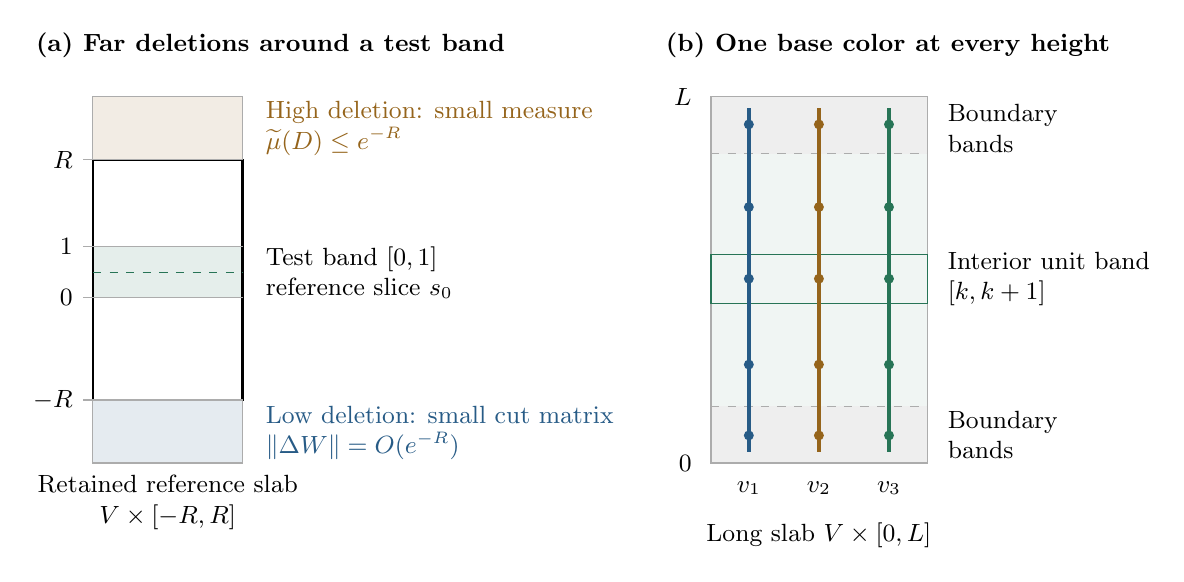
\begin{tikzpicture}[x=1cm,y=1cm,font=\small,
  every node/.style={inner sep=2pt},
  heightline/.style={gray!65,thin},
  fiber/.style={very thick}]
  \definecolor{mahblue}{RGB}{39,91,134}
  \definecolor{mahgold}{RGB}{149,100,27}
  \definecolor{mahgreen}{RGB}{39,116,86}

  \node[anchor=west,font=\small\bfseries] at (0,5.7)
    {(a) Far deletions around a test band};
  \fill[mahgold!12] (.8,4.25) rectangle (2.7,5.05);
  \fill[mahblue!12] (.8,.4) rectangle (2.7,1.2);
  \fill[mahgreen!12] (.8,2.5) rectangle (2.7,3.15);
  \draw[heightline] (.8,.4) rectangle (2.7,5.05);
  \draw[thick] (.8,1.2) rectangle (2.7,4.25);
  \foreach \y/\t in {1.2/{-R},2.5/{0},3.15/{1},4.25/{R}} {
    \draw[heightline] (.68,\y)--(2.7,\y);
    \node[anchor=east] at (.62,\y) {$\t$};
  }
  \draw[dashed,mahgreen] (.8,2.82)--(2.7,2.82);
  \node[anchor=west,align=left,text=mahgold] at (2.92,4.65)
    {High deletion: small measure\\$\widetilde\mu(D)\leq e^{-R}$};
  \node[anchor=west,align=left] at (2.92,2.82)
    {Test band $[0,1]$\\reference slice $s_0$};
  \node[anchor=west,align=left,text=mahblue] at (2.92,.78)
    {Low deletion: small cut matrix\\$\|\Delta W\|=O(e^{-R})$};
  \node[align=center] at (1.75,-.1)
    {Retained reference slab\\$V\times[-R,R]$};

  \node[anchor=west,font=\small\bfseries] at (8,5.7)
    {(b) One base color at every height};
  \fill[gray!13] (8.65,.4) rectangle (11.4,1.12);
  \fill[gray!13] (8.65,4.33) rectangle (11.4,5.05);
  \fill[mahgreen!7] (8.65,1.12) rectangle (11.4,4.33);
  \draw[heightline] (8.65,.4) rectangle (11.4,5.05);
  \draw[heightline,dashed] (8.65,1.12)--(11.4,1.12);
  \draw[heightline,dashed] (8.65,4.33)--(11.4,4.33);
  \draw[mahgreen] (8.65,2.43) rectangle (11.4,3.05);
  \foreach \x/\c in {9.13/mahblue,10.02/mahgold,10.91/mahgreen} {
    \draw[fiber,\c] (\x,.54)--(\x,4.91);
    \foreach \y in {.75,1.65,2.74,3.65,4.7}
      \fill[\c] (\x,\y) circle (1.8pt);
  }
  \node[anchor=east] at (8.48,.4) {$0$};
  \node[anchor=east] at (8.48,5.05) {$L$};
  \node[anchor=west,align=left] at (11.58,4.65) {Boundary\\bands};
  \node[anchor=west,align=left] at (11.58,2.74)
    {Interior unit band\\$[k,k+1]$};
  \node[anchor=west,align=left] at (11.58,.76) {Boundary\\bands};
  \node at (9.13,.08) {$v_1$};
  \node at (10.02,.08) {$v_2$};
  \node at (10.91,.08) {$v_3$};
  \node[align=center] at (10.02,-.52)
    {Long slab $V\times[0,L]$};
\end{tikzpicture}
\caption{Height geometry behind Lemmas~\ref{lem:far-deletion}
and~\ref{lem:coherent-choice} (not to scale). High and low deletions
are controlled by different estimates. A color selected on the
reference slice is used at every height above the same base vertex.
Translated interior unit bands compare with the reference slab in
integrated normalized data; the boundary bands have total length at
most $2R+2$. The colored vertical lines are base fibers
$\{v\}\times[0,L]$, not lifted relation orbits.}
\label{fig:maharam}
\end{figure}

